\documentclass[titlepage, 12pt, a4paper, english]{report}

%%% packages %%%
\usepackage{titling}

\usepackage{graphicx}

\usepackage[backend=biber,citestyle=numeric-comp,bibstyle=numeric]{biblatex}
\addbibresource{./references.bib}

\usepackage{mathptmx}

\usepackage{float}

\usepackage{threeparttable}
\usepackage{tabularx}
\usepackage{adjustbox}
\usepackage{multirow}

\usepackage{pgfplots}
\pgfplotsset{width=10cm,compat=1.9}
\usepgfplotslibrary{external}
%\tikzexternalize %%disabled until I fix it (if I fix it)

\setcounter{secnumdepth}{4}
\setcounter{tocdepth}{4}

\usepackage[version=4]{mhchem}

% We do a bit of trolling :3
\usepackage[T1]{fontenc}
%\usepackage[math]{anttor}

%%% title page %%%
% Do not touch it, it's a mess with a bunch of warnings but it works and looks how it should and I'm afraid trying to fix it would break it too much.
\pretitle{
	\vspace*{-6cm}
  \noindent\makebox[\linewidth][c]{\includegraphics[width=6cm]{z_Assets/Images/Duhovka-logo.png}}
	\par\vspace{1.5cm}
	\centering
	\fontsize{22}{26}\selectfont
}
\posttitle{
	\par
	\vspace{0.5cm}
	\noindent\rule{14cm}{0.4pt}
}    
\title{The Evolution of Rocket Engines and Their Role in Humanity’s Quest for Interstellar Travel}
\author{Filip Rousek\\[0.5em]{\large \emph{Consultant:} Morteza Kerachian}}
\date{October 2025}

%%% document body %%%
\begin{document}
	\maketitle
	
	\section{Prohlášení}
	Prohlašuji, že jsem svoji seminární práci vypracovala samostatně a veškeré použité
	zdroje a další podkladové materiály uvádím v seznamu použitých zdrojů.
	
	\vspace{2em}
	Datum:\hspace{5cm}Podpis:
	
	\tableofcontents
	\newpage
  %% INTRODUCTION & HISTORY %%
  \chapter{Introduction}
    \section{Objectives and Structure of the Work}
      This Seminar work aims to explain and innovate on the rich history of rocket engines we as a civilization have as well as theorize on the possible directions we could improve this in the future.\\
      The paper is structured as follows. Firstly, a brief introduction to the background and motivation of this work and humanity's strive for the stars. Secondly, a theoretical part explaining the basics and different types of engines (both air breathing and combustion) currently in use. Further on a relatively breath walkdown of the historical evolution of rocket engines and lastly some more theoretical projects and frameworks for better, faster and more effective propulsion. Thirdly, a practical part where I utilize NPSS and attempt to improve on current models and design a possible liquid fuel rocket engine, with the results of simulations ran on it. Last, but certainly not least is the conclusion in which I summarize this work and evaluate if it has succeeded in the goals I've set for myself and the results of the practical part.
    \section{Background and Motivation}
      Humanity has looked up at the starry night and wondered “What is out there?” since its beginning. Many cultures, both historically early (before the Common Era) and later (after) have given the sky and stars a significant position in theirreligions. The ancient Egyptians believed that stars were the destinations of souls ascending to the afterlife; Christianity holds concepts of Heaven among or beyond the stars. Other examples include the Babylonians who charted the sky and tied celestial events to divine influence, the Greeks who philosophised about the cosmos, and indigenous peoples whose cosmologies placed humans in relation to the night sky.\\ 
        Since our discovery of flight, many have further wondered: “Could we reach them?”
      \subsection{The era of space}
      The mid-20th century marked a pivotal shift from dreaming about space to actually reaching into it. The colloquially known Space Race between the United States and the Soviet Union was driven by a combination of geopolitical rivalry, technological ambition, and human curiosity. The Soviets launched the first artificial satellite, Sputnik 1, in 1957, initiating the Space Age. In 1961 the Soviets sent Yuri Gagarin into orbit—the first human to travel into space. The United States followed with its Apollo programme, culminating in Apollo 11 landing humans on the Moon in 1969.\\
        Beyond symbolism, the space race demanded the development of new propulsion technologies, materials, life-support systems, and systems engineering. These developments laid the foundation for modern aerospace engineering.\\
        \subsection{Why do we strive for Space?}
        Why has humanity been so drawn to space? In my own opinion, the answer to this question can be distilled into the following inter-related motivations:
        \begin{itemize}
        \item \textbf{Curiosity and the strive for knowledge:} The urge to explore, to understand the cosmos and our place within it, has driven astronomers, engineers and dreamers alike.
        \item \textbf{Survival and expansion:} Some argue that humanity’s long-term survival may require becoming a multi-planet species, especially given planetary risks.
        \item \textbf{Technological and economical value:} Space-based systems (satellites, communications, Earth observation) have become integral to modern life and economies.
        \item \textbf{Inspiration and the search for identity:} Achievements in space serve as proof of human potential, inspiring new generations and influencing cultural identity.
        \end{itemize}
      
        At the heart of all of these reasons lies propulsion technology. To move from Earth orbit to other celestial bodies (or even interstellar destinations) we require efficient, powerful, and reliable propulsion systems. Without them, the dream of reaching the stars remains just that—a dream. Advances in propulsion (chemical rockets, nuclear thermal, electric propulsion, solar sails and beyond) are critical enablers of space exploration, colonisation, and the realisation of humanity’s cosmic ambitions.


        
  \section{A brief history of rocket engines}
  \subsection{Early Concepts and the First Rocket Engine}
    (Briefly cover early gunpowder rockets and pioneers like Tsiolkovsky, Goddard, Oberth.)

  \subsection{The First Rocket to Reach Space}
    The German \textit{Aggregat-4}, better known as the \textit{V-2 rocket}, was the first human-made object to reach the edge of space. Developed under the direction of Wernher von Braun during World War II, the V-2 achieved suborbital altitudes exceeding 80~km in 1944 and was capable of carrying a 1-ton warhead to a range of about 320~km.\supercite{neufeld1995}

    \begin{figure}[H]
      \begin{center}
        \includegraphics[width=0.5\textwidth]{z_Assets/Graphics/Photos/V-2_förbränningskammare.JPG}
      \end{center}
      \caption{Rocket engine used by V-2\supercite{Img_v2-engine}}\label{fig:rocket-engine-v2}
    \end{figure}

    \begin{figure}[H]
      \begin{center}
        \includegraphics[width=0.95\textwidth]{z_Assets/Graphics/Schematics/960px-Esquema_de_la_V-2.jpg}
      \end{center}
      \caption{A U.S. Army cut-away diagram of the V-2\supercite{Img_us-cutaway-v2}}\label{fig:us-army-cutaway-diagram-v2}
    \end{figure}


The V-2 used a liquid-propellant engine burning ethanol and liquid oxygen in a gas-generator cycle, producing roughly 25 metric tons of thrust. Its innovations—including turbopumps, gyroscopic guidance, and regenerative cooling—formed the foundation of post-war rocket programs in both the United States and the Soviet Union. The American Redstone and Jupiter missiles, as well as the Soviet R-7 that launched \textit{Sputnik}, directly descended from V-2 technology.\supercite{neufeld1995}

\begin{figure}[H]
      \begin{center}
        \includegraphics[width=0.5\textwidth]{z_Assets/Graphics/Photos/Rocket_engine_A4_V2.jpg}
      \end{center}
      \caption{A sectioned V-2 engine on display at the Deutsches Museum, Munich (2006)\supercite{Img_sectioned-v2-engine}}\label{fig:}
    \end{figure}
   
    \begin{figure}[H]
  \begin{center}
    \includegraphics[width=0.5\textwidth]{z_Assets/Graphics/Schematics/Aggregat4-Schnitt-engl.jpg}
  \end{center}
  \caption{Layout of a V2 rocket\supercite{Img_v2-layout}}\label{fig:}
\end{figure}

   \subsection{The Saturn V F-1 Engine}
  The engine who got man to the moon upon the widely known Saturn V rocket was the Rocketdyne F-1 gas-generator cycle single combustion chamber liquid-propellant rocket engine.\supercite{young2008}
\\

    It is the most powerful single-nozzle liquid-fueled engine ever used and was placed upon the first stage of Saturn V.\supercite{young2008}
  \begin{table}[H]
  \centering
  \begin{threeparttable}
    \begin{tabular}{|| c | c ||}
      \hline
      \textbf{TYPE} & \textbf{SPECIFICATION} \\
      \hline \hline
      Length & 19ft \\
      \hline
      Width & 12ft 4in \\
      \hline
      Thrust (sea level) & 1,500,000 lbs \\
      \hline
      Specific Impulse (minimun) & 260 sec \\
      \hline
      Rated run duration & 150 sec \\
      \hline
      \multirow{2}{*}{Flowrate} & \textit{Oxidizer: } 3,945 lbs/sec (24,811 gpm) \\
      \cline{2-2}
        &\textit{Fuel: } 1,738 lbs/sec (15,471 gpm)\\
      \hline
      Mixture ratio & 2.27:1 (oxidizer to fuel)\\
      \hline
      Chamber pressure & 965 psia\\
      \hline
      Weight flight configuration & 18,500 lbs maximum\\
      \hline
      \multirow{2}{*}{Expansion area ratio} & \textit{With nozzle extension:} 16:1 \\
      \cline{2-2}
        & \textit{Without nozzle extension:} 10:1\\
      \hline
      \multirow{2}{*}{Combustion temperature} & \textit{Thrust Chamber:} 5,970°F\\
      \cline{2-2}
       & \textit{Gas Generator:} 1,465°F\\
       \hline
      Maximum exit nozzle diameter & 11ft 7in\\
      \hline
  \end{tabular}
  \caption{Technical specifications of the F-1 Engine.\supercite{young2008}}
  \end{threeparttable}
\end{table}
  \subsection{Post-Saturn Developments}
  Following the success of the Saturn~V, rocket propulsion entered a new era marked by reusability, efficiency, and high-performance engines.

\subsubsection{Space Shuttle Main Engine (SSME)}
NASA’s Space Shuttle Main Engine (RS-25) represented a leap in reusable liquid propulsion. It was a staged-combustion hydrogen–oxygen engine capable of being throttled between 65\% and 109\% thrust. Each RS-25 generated about 1.8~MN of thrust and could be reused up to 55 times.\supercite{young2008}

\subsubsection{Soviet and Russian Advances}
In the Soviet Union, engineers developed the RD-170 and its derivatives, the world’s most powerful liquid rocket engines by total thrust (7.9~MN). These engines used a closed-cycle staged combustion process with kerosene and LOX, achieving exceptional efficiency and reliability, later adapted for Zenit and Atlas launch vehicles.\supercite{chertok2012}
\\

\subsubsection{Modern Developments: Merlin and Raptor}
SpaceX’s \textit{Merlin} engines, used on the Falcon 9, utilize RP-1 and LOX in a gas-generator cycle optimized for reusability. The newer \textit{Raptor} engine, employing methane and LOX in a full-flow staged combustion cycle, represents one of the most advanced chemical rocket engines ever built. Its design emphasizes reusability, efficiency, and adaptability for interplanetary missions, particularly SpaceX’s Starship program aimed at Mars colonization.\supercite{spaceX-raptor}

  %% THEORETICAL BACKGROUND %%
   \chapter{Theoretical Part}
         \section{Classification of Propulsion Systems}

    Propulsion is defined as \textit{"the action or process of propelling"} (\textit{"to drive forward or onward by or as if by means of a force that imparts motion"}). By the Merriam-Webster Dictionary. 

    It can also be defined as "the act of changing the motion of a body with respect to an inertial reference frame."\supercite{sutton2017}

    In engine propulsion, the most common way to achieve such thing is via \textit{chemical combustion}. The energy can also be supplied by \textit{solar radiation}, or a \textit{nuclear reactor}. As such, the varios types of propulsion can be generally divided up into three categories:
    \begin{itemize}
        \item chemical propulsion
        \item nuclear propulsion
        \item solar propulsion
    \end{itemize}

   \begin{table}[H]
     \begin{adjustbox}{minipage=\textwidth+135pt, center}
  \centering
  \begin{threeparttable}
    \begin{tabular}{|| c | c | c | c | c ||}
      \hline \hline
      \multirow{2}{*}{\textbf{Propulsion Device}} &
        \multicolumn{3}{| c |}{\textbf{Energy Source}$^a$} &
        \multirow{2}{*}{\textbf{Propellant or Working Fluid}} \\
        \cline{2-4}
      & Chemical & Nuclear & Solar & \\
      \hline
      Turbojet & D/P &  &  & Fuel + air \\
      \hline
      Turbo-ramjet & TFD &  &  & Fuel + air \\
      \hline
      Ramjet (Hydrocarbon fuel) & D/P & TFD &  & Fuel + air \\
      \hline
      Ramjet ($H_2$ cooled) & TFD &  &  & Hydrogen + air \\
      \hline
      Rocket (chemical) & D/P & TFD &  & Stored propellant \\
      \hline
      Ducted rocket & TFD &  &  & Stored solid fuel + surrounding air \\
      \hline
      Electric rocket & D/P &  & D/P & Stored propellant \\
      \hline
      Nuclear fission rocket &  & TFD &  & Stored $H_2$ \\
      \hline
      Solar heated rocket &  &  & TFD & Stored $H_2$ \\
      \hline
      Photon rocket$^b$ &  & TFND &  & Photon ejection (no stored propellant) \\
      \hline
      Solar sail &  &  & TFD & Photon reflection (no stored propellant) \\
      \hline
    \end{tabular}

    \begin{tablenotes}
      \item[a] \textbf{D/P} developed and/or considered practical; 
      \textbf{TFD} technical feasibility has been demonstrated, but development is incomplete; 
      \textbf{TFND} technical feasibility has not yet been demonstrated.
      \item[b] Essentially a really big light bulb. 
    \end{tablenotes}

    \caption{Energy Sources and Propellants for Various Propulsion Concepts\supercite{sutton2017}}
    \label{tab:1-1}
  \end{threeparttable}
\end{adjustbox}
\end{table} 
  

    Input in rocket propulsion systems is either heat or electricity. Useful output thrust comes from the kinetic energy of the ejected matter and from the propellant pressure on inner chamber walls and at the nozzle exit; thus. rocket propulsion systems primarily convert input energies into the kinetic energy of the exhausted gas. The ejected mass can be in a solid, liquid or gaseous state. Often, combinations of two or more states are ejected. At high enough temperatures, the ejected mass can also be in a state of plasma.\supercite{sutton2017}

    \subsection{Duct Jet Propulsion}
      Duct jet engines, more commonly called "air breathing" engines, are engines which utilize airflow that is then energized inside a duct. They use atmospheric oxygen to burn fuel stored onboard. This class includes the following:\supercite{sutton2017}
      \begin{itemize}
          \item turbojets
          \item turbofans
          \item ramjets
          \item pulse jets
          \item scramjets\supercite{segal2009}
      \end{itemize}
      They are mentioned here mainly as to provide a background and comparison to rocket propulsion engines.
      \begin{table}[H]
        \centering

        \begin{threeparttable}
          \begin{tabular}{|| p{3cm} | p{3cm} | p{3cm} | p{3cm} ||}
              \hline
              Feature & Chemical Rocket Engine or Rocket Motor & Turbojet Engine & Ramjet Engine \\
              \hline\hline
              thrust to weight ratio, typical & 75:1 & 5:1, turbojet and afterburner & 7:1 at Mach 3 at 9,144m (30,000ft) \\
              \hline
              Specific fuel consumption$^{a}$ & 8 - 14 & 0.5 - 1.5 & 2.3 - 3.5 \\
              \hline
              Specific thrust$^{b}$ & 5,000 - 25,000 & 2500 (low Mach$^{c}$ numbers at sea level) & 2700 (Mach 2 at sea level) \\
              \hline
              Specific impulse$^{d}$ & 270 sec & 1600 sec & 1400 sec \\
              \hline
              Thrust change with altitude & Slight increase & Decrease & Decrease \\
              \hline
              Thrust vs. flight speed & Nearly constant & Increases with speed & Increases with speed \\
              \hline
              Thrust vs air temperature & Constant & Decreases with temperaure & Decreases with temperature \\
              \hline
              Flight speed vs. exhaust velocity & Unrelated, flight speed can be greater & Flight speed always less than exhaust velocity & Flight speed always less than exhaust velocity \\
              \hline
              Altitude limitation & None; suited for space travel & 14,000 - 17,000 m & 20,000 m at Mach 3, 30,000 m at Mach 5, 45,000 m at Mach 12 \\
              \hline
          \end{tabular}

          \begin{tablenotes}
            \item[a] Multiply by 0.102 to convert to $kg/(hr-N)$.
            \item[b] Multiply by 47.9 to convert to $N/m^2$
            \item[c] Mach number is the ratio of gas speed to local speed of sound (See Equation~\ref{eq:Mach Number}(Appendix~\ref{app:equations})).
            \item[d] \textit{Specific impulse} is a performance parameter (See Equation~\ref{eq:Specific Impulse}(Appendix~\ref{app:equations})) 
            \end{tablenotes}

          \caption{Comparison of Several Characteristics of a Typical Chemical Propulsion Rocket Propulsion System and Two-Duct Propulsion Systems\supercite{sutton2017}} 
          \label{tab:1-2}
          \end{threeparttable}
        \end{table}


      Out of all of the ducted engines, the \textit{turbojet engine} is the most widely used.

    \subsubsection{Ramjet Engine}
      For supersonic flight in the speeds above Mach 2, the \textit{ramjet engine} (which is a pure ducted engine) is the best suited within the earth's atmosphere. Its compression is purely gas dynamic and thrust is produced by increasing the momentum of the subsonic compressed air as it passes through the ramjet in a very similar manner to the functionality of \textit{turbofan} and \textit{turbojet} engines, just without any compressor or turbine hardware.\supercite{sutton2017} 

      \begin{figure}[H]
        \centering
        \includegraphics[width=0.75\linewidth]{z_Assets/Graphics/Schematics/Ramjet_P280b.jpg}
        \caption{Simplified schematic of a ramjet engine with a supersonic inlet (a converging/diverging flow passage)\supercite{Nasa_ramjet-schematic}}
        \label{fig:ramjet engine}
      \end{figure}

      Ramjets with subsonic combustion and hydrocarbon fuels have an upper speed limit of approx. 5 Mach; Hydrogen fuel with hydrogen cooling raises this maximum to at least 16 Mach.

    \subsubsection{Scramjet Engine}
      The Scramjet engine is a ramjet engine utilizing \textit{super sonic combustion}. Which allows for much freeer and faster air flow than \textit{turbojet} or \textit{ramjet} engines.
      \begin{figure}[H]
        \centering
        \includegraphics[width=0.5\linewidth]{z_Assets/Graphics/Schematics/Turbo_ram_scramjet_comparative_diagram.svg-1.png}
        \caption{The compression, combustion, and expansion regions of: \textbf{(a)} turbojet, \textbf{(b)} ramjet, and \textbf{(c)} scramjet engines.\supercite{Img_scramjet}}
        \label{fig:scramjet engine_comparison}
      \end{figure}
      So far, Scramjet engines have only been used in a few prototype vehicles and military experiments. A Scramjet relies on high vehicle speed to compress the incoming air forcefully before combustion (hence sc (\textit{supersonic combustion}) \textbf{ramjet}), but whereas a ramjet decelerates the air to subsonic velocities before combustion using shock cones, a Scramjet has no shock cone and slows the airflow using shockwaves produced by its ignition source in place of a shock cone.\supercite{segal2009}${}^;$\supercite{Wiki_scramjet}



      \subsection{Rocket Propulsion}
      Rocket propulsion is based fundamentally on \textit{Newton’s Third Law of Motion} — for every action, there is an equal and opposite reaction. In a rocket engine, the “action” is the high-velocity expulsion of exhaust gases, while the “reaction” propels the vehicle forward. Unlike air-breathing engines, rockets carry both fuel and oxidizer, allowing them to function in the vacuum of space.\supercite{sutton2017}

\subsubsection{Chemical Rocket Engines}
Chemical propulsion remains the most widely used method of achieving thrust in spaceflight. It relies on the combustion of chemical propellants that release large amounts of thermal energy, which is converted into kinetic energy of the exhaust gases. Two major types exist: \textit{solid} and \textit{liquid} rocket engines.\supercite{sutton2017}

\paragraph{Solid Rocket Engines}
Solid rocket motors use propellants in a single solid mixture, often consisting of a powdered oxidizer (such as ammonium perchlorate) combined with a binder that also acts as fuel. They are mechanically simple, capable of long storage, and deliver high thrust rapidly after ignition. However, they cannot be throttled or shut down once ignited, limiting flexibility.\supercite{sutton2017}

\begin{figure}[H]
  \begin{center}
    \includegraphics[width=0.5\textwidth]{z_Assets/Graphics/Schematics/Solid-Fuel_Rocket_Diagram.png}
  \end{center}
  \caption{A simplified diagram of a solid-fuel rocket.
    \textbf{(1)} A solid fuel-oxidizer mixture (propellant) is packed into the rocket, with a cylindrical hole in the middle.
    \textbf{(2)} An igniter combusts the surface of the propellant.
    \textbf{(3)} The cylindrical hole in the propellant acts as a combustion chamber.
    \textbf{(4)} The hot exhaust is choked at the throat, which, among other things, dictates the amount of thrust produced.
  \textbf{(5)} Exhaust exits the rocket.
  \supercite{Img_solid-rocket-fuel}
}\label{fig:solid-fuel-rocket-diagram}
\end{figure}

\paragraph{Liquid Rocket Engines}
Liquid-propellant engines store the oxidizer and fuel in separate tanks and feed them into a combustion chamber using pumps or pressurization. The most common combinations are RP-1 (refined kerosene) with liquid oxygen (\ce{LOX}), or liquid hydrogen (\ce{LH2}) with \ce{LOX}. They can be throttled, restarted, and provide high efficiency but require complex plumbing and cryogenic storage.\supercite{sutton2017}

\begin{figure}[H]
  \begin{center}
    \includegraphics[width=0.5\textwidth]{z_Assets/Graphics/Schematics/Liquid-Fuel_Rocket_Diagram.png}
  \end{center}
  \caption{A simplified diagram of a liquid-propellant rocket.
    \textbf{(1)} Liquid rocket fuel.
    \textbf{(2)} Oxidizer.
    \textbf{(3)} Pumps carry the fuel and oxidizer.
    \textbf{(4)} combustion chamber mixes and burns the two liquids.
    \textbf{(5)} Combustion product gasses enter the nozzle through a throat.
  \textbf{(6)} Exhaust exits the rocket.\supercite{Img_liquid-rocket-fuel}}\label{fig:liquid-fuel-rocket-diagram}
\end{figure}

\paragraph{Hybrid Rocket Engines}
A hybrid rocket uses a combination of a liquid oxidizer and a solid fuel. This design offers a compromise between the safety of solid motors and the controllability of liquid systems. Notable examples include SpaceShipOne’s nitrous oxide (\ce{N2O}) and hydroxyl-terminated polybutadiene (\ce{HTPB}) hybrid engine.\supercite{sutton2017}

\begin{figure}[H]
  \begin{center}
    \includegraphics[width=0.75\textwidth]{z_Assets/Graphics/Schematics/SpaceShipOne_schematic.png}
  \end{center}
  \caption{Hybrid rocket motor detail of SpaceShipOne\supercite{Img_spaceshipone}}\label{fig:hybrid-rocket-motor-spaceshipone}
\end{figure}

\subsubsection{Non-Chemical Rocket Engines}
Beyond chemical propulsion, various non-chemical systems have been developed to improve efficiency and endurance for deep-space missions.

\paragraph{Electric Propulsion}
Electric propulsion systems, such as ion and Hall-effect thrusters, use electrical energy (from solar arrays or nuclear sources) to accelerate charged particles. They produce low thrust but extremely high specific impulse, making them ideal for long-duration missions where gradual acceleration is acceptable.\supercite{sutton2017}

\paragraph{Nuclear Thermal Propulsion (NTP)}
In nuclear thermal systems, a nuclear reactor heats a propellant—typically hydrogen—to extremely high temperatures before expansion through a nozzle. This method can theoretically double the specific impulse compared to chemical rockets, offering a promising balance between power and efficiency for interplanetary travel.\supercite{sutton2017}
  \section{Emerging Propulsion Technologies}
    % (Ion engines, nuclear thermal propulsion, solar sails, and antimatter or fusion concepts.)
    As mentioned at the beginning of this work, there still are ideas and possible engines that have yet to depart the zone of science fiction as either our technology isn't advanced enough to produce and test such engines or they have been demonstrated to not be technically effective for their complexity/price or we have no use for them yet. I shall talk about a select few of these in the following parts. Mainly the following:
    \begin{itemize}
      \item Nuclear Propulsion (both Fusion and Fission)
      \item Ion Engines 
      \item Solar Sails
      \item Antimatter Engines
      \item Field Propulsion
    \end{itemize}

    \subsection{Nuclear Propulsion}
    \subsubsection{Fusion}
    \subsubsection{Fission}

    \subsection{Ion Engines}

    \subsection{Solar Sails}

    \subsection{Antimatter Engines}

    \subsection{Field Propulsion}
  Field propulsion, as defined by Yoshinari Minami is the act of propulsion not by usual means of momentum thrust, but instead by pressure thrust derived from an interaction of a spaceship with the physical structure of space-time. (Assuming that space as a vacuum possesses a substantial physical structure.)\supercite{minami2018}\\

    As the theory stands, field propulsion remains speculative and has not yet been experimentally demonstrated. It arises from the idea that spacetime itself may be manipulated to create a net force on a spacecraft without the expulsion of reaction mass. Concepts such as the \textit{Alcubierre warp drive}, derived from solutions to Einstein’s field equations, suggest that spacetime could theoretically be contracted in front of and expanded behind a spacecraft, allowing apparent faster-than-light travel.\supercite{minami2018}

    However, the energy requirements are currently astronomical, exceeding the mass–energy of entire planets, and the feasibility of generating negative energy densities remains purely theoretical. Despite these limitations, research into quantum vacuum interactions and general relativistic field manipulation continues at a conceptual level, keeping the idea alive in advanced propulsion discussions.\supercite{minami2018}


  \section{Theoretical Framework for Interstellar Propulsion}
    Interstellar travel demands propulsion technologies far beyond current chemical or even nuclear capabilities. Several theoretical and conceptual projects have proposed methods to achieve fractions of the speed of light.

\subsection{Project Daedalus}
Conceived in the 1970s by the British Interplanetary Society, \textit{Project Daedalus} proposed a two-stage fusion-powered spacecraft capable of reaching 12\% the speed of light. It would use pellets of deuterium and helium-3 ignited by electron beams to produce thrust. Though technologically beyond current reach, Daedalus provided a credible engineering framework for interstellar flight.\supercite{project_daedalus_propulsion}

\subsection{Breakthrough Starshot}
A modern descendant of the Daedalus concept, \textit{Breakthrough Starshot} envisions launching gram-scale probes accelerated by ground-based laser arrays to 20\% the speed of light. The probes would use lightweight sails reflecting focused laser beams, allowing rapid travel to nearby stars like Proxima Centauri within a human lifetime.\supercite{Wiki_breakthrough_starshot}

\subsection{The Alcubierre Drive}
Proposed by Miguel Alcubierre in 1994, the \textit{warp drive} concept relies on the manipulation of spacetime geometry, compressing space ahead of the craft and expanding it behind. This would allow effective faster-than-light travel without violating local relativistic constraints. Nonetheless, it requires exotic matter with negative energy density, which has not been observed in usable quantities.\supercite{alcubierre1994}
\\

These speculative frameworks demonstrate the profound link between physics and engineering in the pursuit of interstellar travel, emphasizing that humanity’s ultimate propulsion systems may rely as much on breakthroughs in fundamental science as on technological advancement.

\section{Rocket physics fundamentals}
\subsection{Specific Impulse}
      The \textit{specific impulse $I_s$} represents the thrust per unit propellant "weight" flow rate. It is an important figure of merit of the performance of any rocket propulsion system, a concept similar to kilometers per liter or miles per hour as applied to an automobile. A higher number often indicates a better performance. If the total propellant mass flow rate is $\dot{m}$ and the standard acceleration of gravity is $g_0$ (with an \textit{average} value at the Earth's sea level of $9.8066\ m/sec^2$ or $32.174\ ft/sec^2$), then 
      \begin{equation} \label{eq:Specific Impulse}
        I_s = \frac{\int_{0}^{t}Fdt}{g_{0} \int_0^t \dot{m}dt}
      \end{equation}

\subsection{Escape velocity}
Escaoe velocity can be defined as "the minimum speed needed for an object to escape from contact with or orbit of a primary body, assuming:
\begin{itemize}
  \item Ballistic trajectory (no other forces are acting on the object, such as propulsion or friction).
  \item No other gravity-producing objects exist."
\end{itemize}
while the term "velocity" is used colloquially, a more accurate represntation would be "speed" as it is independent of direction.
Escape speed at a distance d from the center of a spherically symmetric primary body (such as a star or a planet) with mass M is given by the formula:
$$
v_e = \sqrt{\frac{2GM}{d}} = \sqrt{2gd}
$$
where:
\begin{itemize}
  \item $G$ is the universal gravitational constant ($G\approx 6.67\times 10^{-11}m^3\times kg^{-1}\times s^{-2}$)
  \item $g = GM/d^2$ is the local gravitational acceleration (or the surface gravity, when d = r).
\end{itemize}
The value $GM$ is called the \textit{gravitational standard parameter}, or $\mu$.
When given an initial speed $V$ greater than the escape speed $v_e$, the object will asymptotically approach the hyperboflic excess speed $v_{\infty}$, satisfying the equation:
$$
v_{\infty}^2 = V^2 - v_e^2
$$
for example, with the definitional value for standard gravity of $9.80665 m/s^2$, the escape velocity for Earth is $11.186\ km/s\ (40,270\ km/h)$.\supercite{Wiki_escape-velocity}
\subsection{Tsoilkovsky's Rocket Equation}
Also called the \textit{Classical Rocket Equation} or \textit{Ideal Rocket Equation}. It describes the motion of vehicles based on the concept of a rocket, defined as "a device that can apply acceleration to itself using thrust by expelling part of its mass with high velocity and can thereby move due to the conservation of momentum".\supercite{Wiki_tsiolkovskys-equation}\\
The maximum change of velociry of thr rocket, $\Delta v$ (with no extrenal forces acting) is:
$$
\Delta v = v_e ln \frac{m_0}{m_f} = I_{sp}g_0 ln\frac{m_0}{m_f}
$$
where:
\begin{itemize}
  \item $v_e$ is the effective exhaust velocity (also equal to $I_{sp}g_0$)
    \begin{itemize}
      \item $I_{sp}$ is the specific impulse in the dimension of time
      \item $g_0$ is standard gravity
    \end{itemize}
  \item $ln$ is the natural logarithm function
  \item $m_0$ is the initial total mass, including propellant (i.e. "wet mass")
  \item $m_f$ is the final total mass, excluding propellant (i.e. "dry mass")
\end{itemize}

Due to the effective exhaust velocity being determined by rocket engine's design, the desired $\Delta v$ (e.g. orbital speed, or escape velocity), and a given dry mass ($m_f$), the equation can be solved for the required wet mass ($m_0$):
$$
m_0 = m_{f}e^{\Delta v/v_e}
$$
The required propellant mass is then: 
$$
m_0 - m_f = m_f(e^{\Delta v/v_e}-1)
$$
This shows us, as can be seen in Figure~\ref{fig:massratio_vs_exhaustratio}, that the nescessary wet mass grows exponentionally with the desired $\Delta v$.\supercite{Wiki_tsiolkovskys-equation}
\begin{figure}[H]
  \centering
  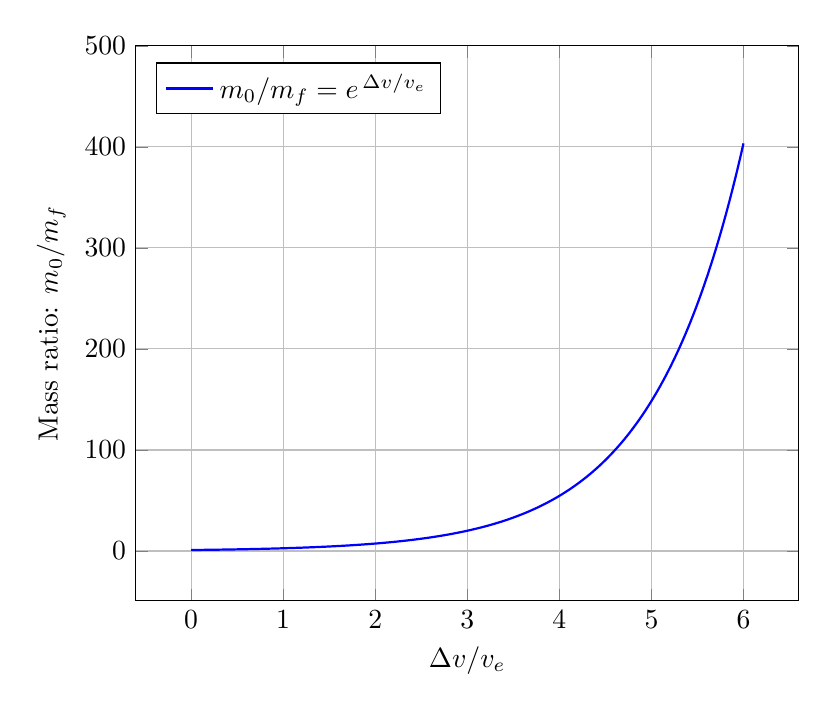
\begin{tikzpicture}
    \begin{axis}[
      xlabel={\(\Delta v / v_e\)},
      ylabel={Mass ratio: \(m_0/m_f\)},
      domain=0:6,
      samples=200,
      grid=major,
      log basis y = e,
      ymax=500,
      legend pos=north west
    ]
      \addplot[blue, thick] {exp(x)};
      \addlegendentry{\(m_0/m_f = e^{\,\Delta v / v_e}\)}
    \end{axis}
  \end{tikzpicture}
  \caption{Required mass ratio as a function of effective exhaust velocity ratio \(\Delta v/v_e\).\supercite{Wiki_toilkovskys-equation}}
  \label{fig:massratio_vs_exhaustratio}
\end{figure}

\subsection{Coriolis Force}
Also known as the \textit{Coriolis effect}, the Coriolis force is a pseudo force that acts on objects in motion within a frame of reference that rotates with respect to an inertial frame. In a reference frame with clockwise rotation, the force acts to the left of the motion of the object. In one with anticlockwise (or counterclockwise) rotation, the force acts to the right. Deflection of an object due to the Coriolis force is called the Coriolis effect. \supercite{Wiki_coriolis-force}

In Newtonian mechanics, the equation of motion for an object in an inertial reference frame is:
$$
F = ma
$$
where $F$ is the vector sum of the physical forces acting on the object, $m$ is the mass of the object and $a$ is the acceleration of the object relative to the inertial reference frame. Transforming this equation to a reference frame rotating about a fixed axis through the origin with angular velocity $\omega$ having variable rotation rate, the equation takes the 
following form:
$$
F' = F-m\frac{d\omega}{dt}\times r'-2m\omega\times v' - m\omega\times (\omega\times r')
$$
where the prime ($'$) variables denote coordinates of the rotating reference frame (not a derivative) and: 
\begin{itemize}
  \item $F$ is the vector sum of the physical forces acting on the object.
  \item $\omega$ is the angular velocity of the rotating reference frame relative to the inertial frame.
  \item $r'$ is the position vector of the object relative to the rotating reference frame. 
  \item $v'$ is the velocity of the object relative to the rotating reference frame.
  \item $a'$ is the acceleration of the object relative to the rotating reference frame.
\end{itemize}
The fictitious forces as they are perceived in the rotating frame act as additional forces that contribute to the apparent acceleration just like the real external forces. The fictitious force terms of the equation are, reading from left to right:
\begin{itemize}
  \item Euler force: $-m\frac{d\omega}{dt}\times r'$
  \item Coriolis force: $-2m(\omega\times v')$
  \item Centrifugal force: $-m\omega\times(\omega\times r')$
\end{itemize}
As seen in these formulas the Euler and centrifugal forces depend on the position vector ($r'$) of the object, while the Coriolis force depends on the object's velocity ($v'$) as measured in the rotating reference frame. As expected, for a non-rotating inertial frame of reference ($\omega = 0$) the Coriolis force and all other fictitious forces disappear.

\subsection{Nozzle flow and geometry}
Rocket engine nozzles, also called propelling nozzles. They are usually of de Laval type (See Figure~\ref{fig:de-laval-nozzle}) used in a rocket engine to expand and accelerate combustion products to high supersonic velocities.\supercite{Wiki_rocket-nozzle}${}^;$\supercite{doi:10.1021/acsomega.1c07050}

Typically, the design of a nozzle aims to achieve maiximum thrust coefficient ($C_F$) potential, which acts as a strong multiplier to the exhaust velocity inherent to the combustion chamber alone (it's characteristic velocity ($c^*$, which is independent of nozzle design).\supercite{Wiki_rocket-nozzle}
\begin{figure}[H]
  \begin{center}
    \includegraphics[width=0.65\textwidth]{z_Assets/Graphics/Schematics/De_laval_nozzle.png}
  \end{center}
  \caption{A de Laval nozzle, showing approximate flow velocity increasing from green to red in the direction of flow\supercite{Img_de-laval-nozzle}}\label{fig:de-laval-nozzle}
\end{figure}

The analysis of gas flow through de Laval nozzles involves a number of concepts and simplifying assumptions:
\begin{itemize}
  \item The combustion gas is an ideal gas.
  \item The gas flow is isentropic.
  \item The gas flow rate is constant during the period of the propellant burn.
  \item The gas flow rate is non-turbulent and axisymmetric from gas inlet to exhaust gas exit.
  \item The flow is compressible as the fluid is a gas.
\end{itemize}

As the combustion gas enters the rocket nozzle, it is traveling at subsonic velocities. As the throat constricts, the gas is forced to accelerate until at the nozzle throat, where the cross-sectional area is the least, the linear velocity becomes sonic. From the throat the cross-sectional area then increases, the gas expands and the linear velocity becomes progressively more supersonic.

The linear velocity of the exiting exhaust gases can be calculated using the following equation:
$$
v_e = \sqrt{\frac{TR}{M}\times\frac{2\gamma}{\gamma - 1}[1-(\frac{p_e}{p})^{\frac{\gamma -1}{\gamma}}]}
$$



  %% IS INtERSTELLAR TRAVEL POSSIBLE? %%
  %\chapter{The quest for Interstellar Travel}
 %%NOTE: SOČ prep %%
  %% DESIGNING A LIQUID PROPELLANT ROCKET ENGINE %%
  \chapter{Practical Part}
   \section{Methodics}
In this practical part I will use the software  \textit{Numerical Propulsion System Simulation} (NPSS) to design a liquid‑propellant rocket engine.  
The aim is to follow a clear, ordered method so that the engine model is built, simulated, and analysed step by step.

\begin{enumerate}
  \item \textbf{Define the design requirements}
    \begin{itemize}
      \item Choose the engine’s purpose (for example: first stage of a launch vehicle, sea‑level take‑off).  
      \item Select the propellants (for example RP‑1 + LOX, or \ce{LH2} + LOX).  
      \item Set the main targets: thrust (in Newtons or kN), burn time (seconds), maximum allowable engine mass, and operating environment (sea level vs vacuum).
    \end{itemize}

  \item \textbf{Select the engine cycle \& make initial assumptions} 
    \begin{itemize}
      \item Decide on the engine cycle type (gas‑generator, staged‑combustion, etc.).  
      \item Make initial assumptions: chamber pressure, mixture ratio (oxidiser : fuel), expansion ratio of the nozzle.  
      \item Note constraints: engine size, material limits, cooling, manufacturability.
    \end{itemize}

  \item \textbf{Build the NPSS model}
    \begin{itemize}
      \item Set up NPSS with the main components: feed system, pumps/turbines, combustion chamber, nozzle.  
      \item Input the assumed parameters: mass flows, pressures, temperatures, geometry (for example throat area, exit area).  
      \item Run the simulation for the “design‑point” (the normal operating condition).
    \end{itemize}

  \item \textbf{Analyse the design‑point results}
    \begin{itemize}
      \item Extract performance data: thrust, specific impulse ($I_{\!sp}$), propellant mass flow, chamber and nozzle pressures and temperatures.  
      \item Compare the results with your design targets from Step 1. If the targets are not met, return to Step 2 (adjust assumptions) or Step 3 (modify model) and iterate.
    \end{itemize}

  \item \textbf{Perform parametric / sensitivity studies}
    \begin{itemize}
      \item Vary one parameter at a time (for example mixture ratio, chamber pressure, expansion ratio) and see how performance changes.  
      \item Record which parameters have the largest effect (sensitivity) and find trade‑offs (for example higher chamber pressure improves $I_{\!sp}$ but may increase mass or cost).  
      \item Use these findings to refine your design toward a better balance.
    \end{itemize}

  \item \textbf{Check off‑design / operating range conditions}
    \begin{itemize}
      \item Use NPSS to simulate the engine under different conditions: for example different ambient pressures (sea level vs high altitude), partial throttle or start‑up conditions.  
      \item Determine how performance changes under these conditions: does thrust drop? does $I_{\!sp}$ fall? Are there stability problems?
    \end{itemize}

  \item \textbf{Document and reflect on the results}
    \begin{itemize}
      \item Prepare tables and graphs presenting your results (design point outputs, parametric study results).  
      \item Discuss your assumptions (for example: ignoring cooling losses, assuming ideal pumps) and their impact.  
      \item Reflect on what I would do differently if you had more time or resources, and what the limits of my design are.
    \end{itemize}
\end{enumerate}

	%% CONCLUSION %%
  \chapter{Conclusion}

\section{Overview}
The aim of this work was to explore how rocket engines have developed over time and how their evolution shapes humanity’s prospects for interstellar travel. The thesis combined three parts: a historical overview, a theoretical explanation of propulsion systems and rocket physics, and a conceptual analysis of what would be required for a rocket engine to reach roughly 1\% of the speed of light.

\section{Key Findings}

\subsection{Historical Perspective}
From early gunpowder rockets to the V-2, Saturn V, and modern engines such as Merlin and Raptor, the history of rocket propulsion shows steady progress toward higher efficiency, improved reliability and, more recently, reusability. Each technological step broadened the range of missions achievable by human-made spacecraft.

\subsection{Theoretical Insights}
The theoretical section showed that propulsion systems differ greatly in capability and purpose. Chemical engines remain unmatched for launch, yet their specific impulse is ultimately limited by chemistry. Concepts such as nuclear propulsion, electric engines, solar sails or even field propulsion offer far higher potential efficiencies, but most remain technically immature or purely speculative. The Tsiolkovsky equation clearly illustrates the core challenge: achieving high $\Delta v$ requires either extremely high exhaust velocities or exponential growth in propellant mass.

\subsection{Conceptual Analysis}
The conceptual analysis applied these principles to the target of achieving a $\Delta v$ of approximately $1\%c$. Even under simplified assumptions and a favourable mass ratio, the required exhaust velocity was found to be on the order of one million metres per second. Scaling a modern chemical engine, such as the Raptor, by any realistic factor does not approach these velocities. This reinforces the conclusion that chemical propulsion cannot serve as a basis for interstellar travel.

\section{Evaluation of Objectives}
Although the initial plan envisioned a simulated practical design, the conceptual approach proved sufficient to meet the core objectives: reviewing historical developments, explaining propulsion theory, and assessing the feasibility of high‐velocity travel. The simplified analysis still demonstrates the physical limits of current engine technology in a clear and meaningful way.

\section{Limitations and Future Work}
The study relied on idealised assumptions, steady-state operation and simplified mass models. No full vehicle architecture or detailed engine cycles were evaluated. Future work could focus on realistic modelling of nuclear or beamed propulsion concepts, or on examining the engineering challenges behind high-energy propulsion systems.

\section{Final Remarks}
Rocket propulsion has taken humanity from simple fireworks to reusable orbital launch vehicles in a historically short time. Yet interstellar travel remains far beyond the reach of current technology. The path forward will depend on breakthroughs in physics and energy generation rather than incremental improvements to chemical engines. Even so, the steady progress of propulsion engineering gives reason to believe that the dream of reaching the stars may eventually move from theory to reality.



  Thank you for taking the time to read this work.
  To end the paper on a light note, I'd like to present to you a rather amusing "meme" in the form of a photoshopped Twitter (X) post.
  \begin{figure}[H]
    \begin{center}
      \includegraphics[width=0.95\textwidth]{z_Assets/Images/meme.png}
    \end{center}
    \caption{A heavily edited picture of a "Tweet" by Konstaltin Tsiolkovsky regarding his famous Rocket Equation, posed in an amusing memetic format.}
  \end{figure}
  
          
      \defbibfilter{papers}{
      type=article or
      type=book
      }
 
      \printbibliography[filter=papers, title={Book and Article Sources}]

    \printbibliography[type=online, title={Online Sources}]

    \printbibliography[type=misc, title={Miscellaneous Sources}]

    \printbibliography[type=image, title={Images}]

\end{document}
